% Copyright (c)  2005-2010 EDF-EADS-PHIMECA.
% Permission is granted to copy, distribute and/or modify this document
% under the terms of the GNU Free Documentation License, Version 1.2
% or any later version published by the Free Software Foundation;
% with no Invariant Sections, no Front-Cover Texts, and no Back-Cover
% Texts.  A copy of the license is included in the section entitled "GNU
% Free Documentation License".

\subsection{Operating principle of a \index{wrapper}wrapper}

\subsubsection{Why use a \index{wrapper}wrapper?}

Among the goals that the \OT\ platform attempts to reach, genericity is central. It is at the heart of the tool as it is at the heart of mathematics, which is the source of all the implemented algorithms. Therefore, an essential part of \OT\ implies that the problem to be solved, and for which we wish to conduct an uncertainty study, can be modeled as a mathematical $\R^{n} \to \R^{p}$ \index{function}function.

This model, which we chose to call \index{Function}Function, can be implemented in various ways.

It can be directly encoded within the library that forms the base of the platform. Currently, and even if it is easily feasible, no \index{Function}Function belongs to this category. The reason is primarily practical. Which Function can be hard-coded? Why this one rather than another? Given that the tool is generic and meant to be broadly disseminated, a choice made for our needs could be a problem in another context. This is why we refused to register the Functions at the library level.

It can also be coded within an analytical formula driven by a \index{NumericalMathFunction}NumericalMathFunction. This\index{data structure} will not be detailed here. It suffices to know that the said analytical formula is not hard-coded but passed as an argument of the NumericalMathFunction, which is able to interpret and execute it. Thus, the platform can work with almost any formula given by the user.

Advancing still further towards the externalization of the computation from the library, the \index{Function}Function can be implemented in a subroutine that will be dynamically (i.e. on demand) linked to the platform during computation.

Finally, it is possible to use this subroutine not to perform the computation, but to delegate this computation to an external entity, that is to say, a computational code (see Figure 3.1).

\begin{figure}
  \begin{center}
    \ifpdf
    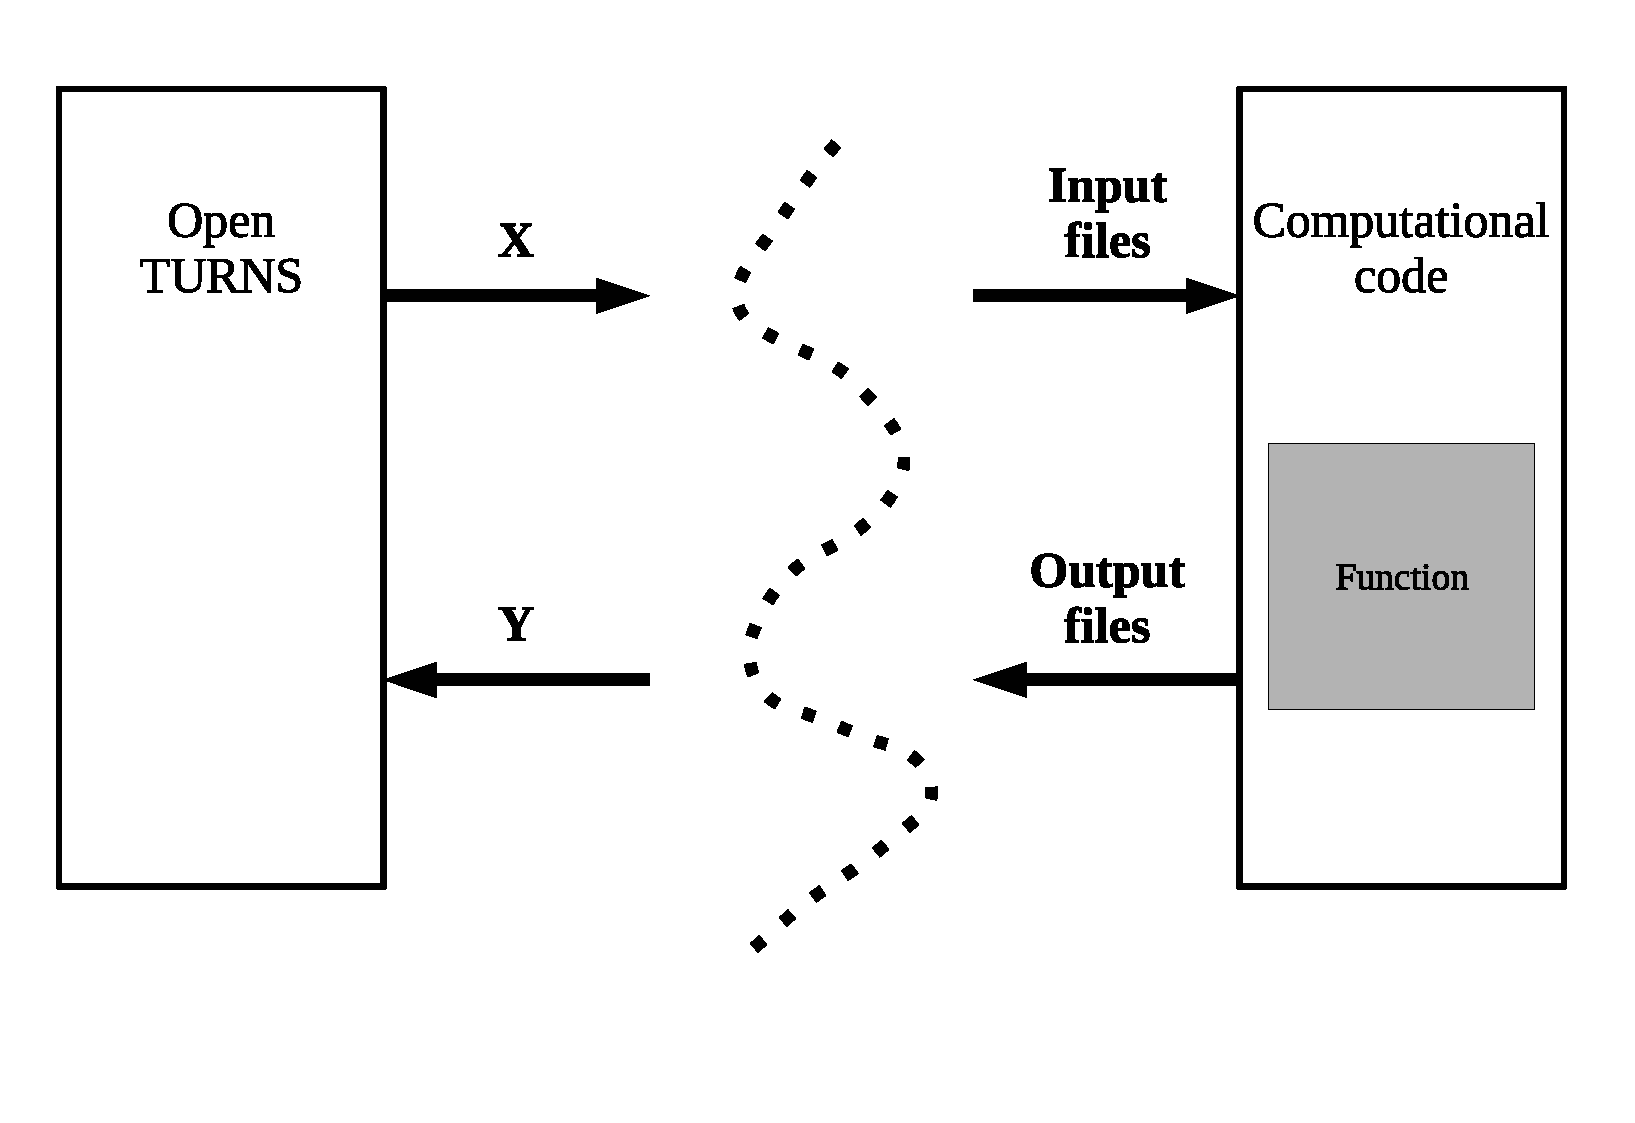
\includegraphics[width=12cm]{Figure1.pdf}
    \else
    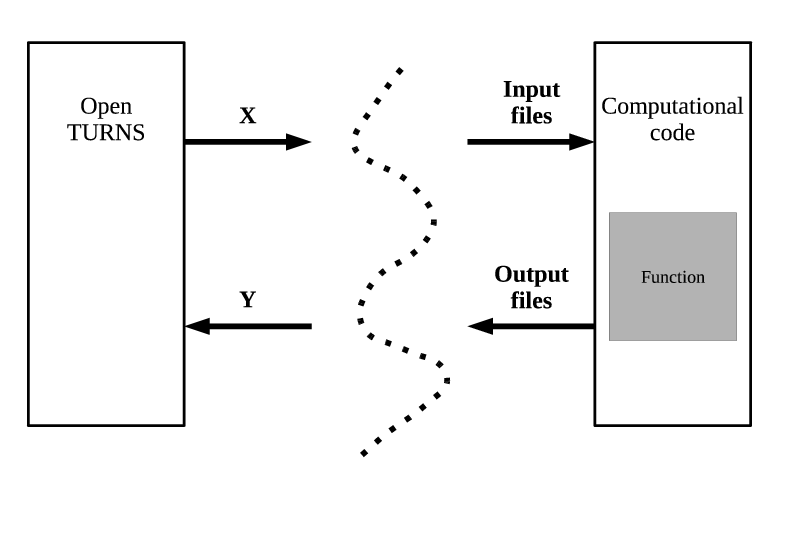
\includegraphics[width=12cm]{Figure1.png}
    \fi
    \caption[Figure 1]{Adapting the interface between \OT\ and the computational code}
  \end{center}
\end{figure}

We are therefore in a situation in which \OT\ only sees the \index{Function}Function hosted within the computational code as an object consuming a set of $n$ values (a vector \underline{X} belonging to $\R^{n}$) and producing a set of $p$ values (a vector \underline{Y} belonging to $\R^{p}$), while the computational code usually expects to receive input files and produce output files.

These files contain much more information than the $n$ or $p$ values manipulated by \OT. Moreover, they have a \index{regular expression}format that is specific to each computational code.

Therefore, it is difficult or even impossible for \OT\ adapt to all situations. It is not possible either to impose a coupling mode and force the computational codes to follow it.

If we look closer, we notice that, on the one hand, \OT\ expects the computational code to respect its interface, that is to say that it transmits the values through vectors \underline{X} and \underline{Y} and that, on the other hand, the computational code expects \OT\ to send values through its interface, that is to say its files.

The \index{wrapper}"wrapper" is precisely the subroutine that converts the interface of one element into an interface of the other, carrying out the necessary transformations on the data. In this document, we will use the word wrapper, although we could also use the more explicit but less common term "interface adapter" (see Figure 3.2).

\begin{figure}
  \begin{center}
    \ifpdf
    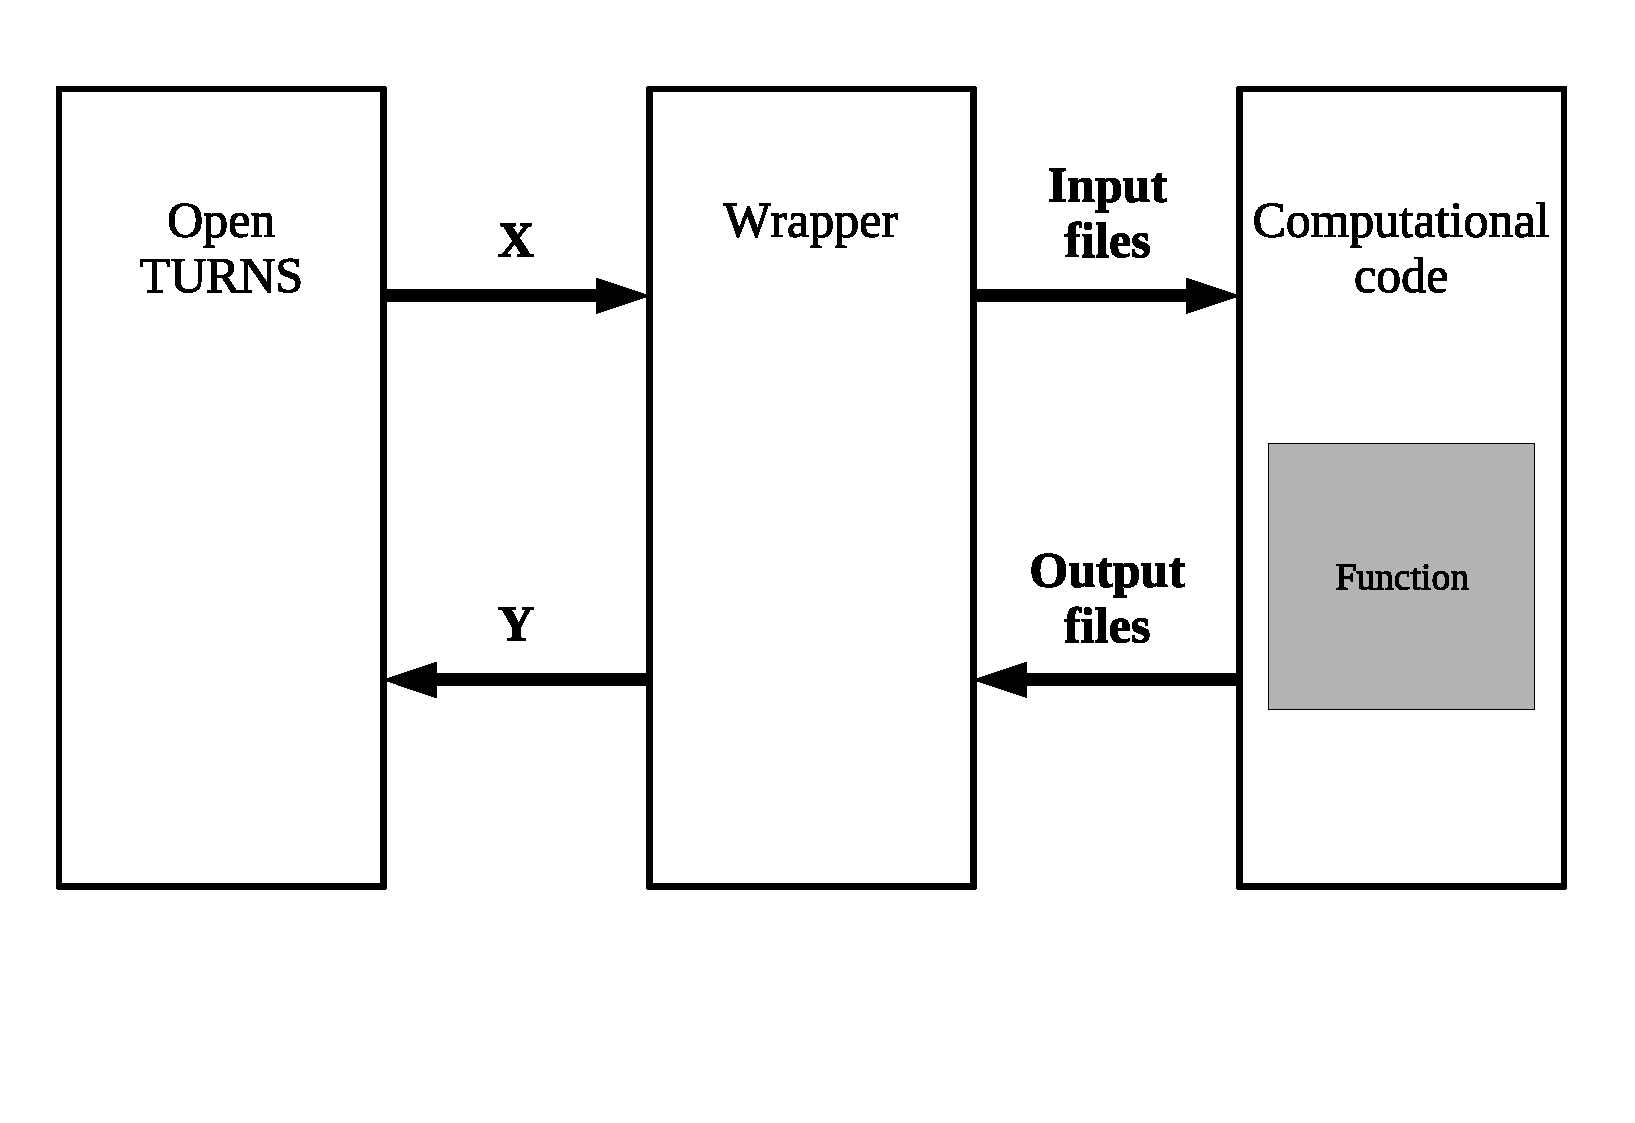
\includegraphics[width=12cm]{Figure2.pdf}
    \else
    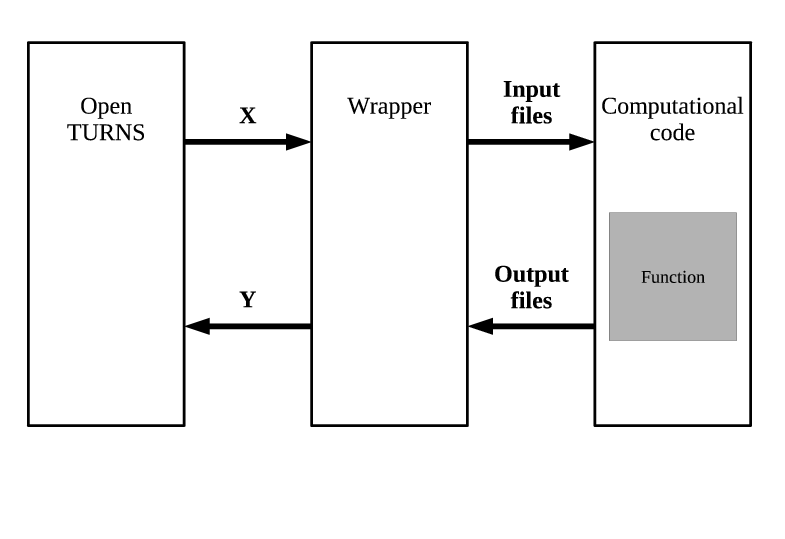
\includegraphics[width=12cm]{Figure2.png}
    \fi
    \caption[Figure 2]{Coupling a computational code using a \index{wrapper}wrapper}
  \end{center}
\end{figure}

Of the three scenarios outlined above, the \index{wrapper}wrapper is only involved in the last two. This document therefore only addresses these two cases.

As an adapter, the \index{wrapper}wrapper is not meant to change the way the user sees the computational code with which they are working. The wrapper should thus be transparent in the exchange between \OT\ and the external code. It behaves as an extension of the code towards the platform.

Beyond its role of interface adaptation, the wrapper also ensures the cooperation between a platform written in C++ and codes written in any other programming language (C, \index{FORTRAN}FORTRAN 77 or 90, Python, etc.). This\index{data structure} will be detailed later on in this document.

It is also in charge of managing the \index{execution}execution of the computational code by invoking its commands or functions at the appropriate time.

In summary, the \index{wrapper}wrapper is a variable geometry interconnection element between \OT\ and the computational code. It can be designed to provide basic or very advanced functionalities. Being specific to each code, it is its designer's responsibility to determine its capabilities.

This documentation is structured following a gradual progression. It begins by showing how to create a minimal \index{wrapper}wrapper with the most basic behavior, which will, however, be adequate in many cases; then, as the reader advances in the text, they will be able to see how to add features enriching the interface. This progression can also be regarded as a design guide for the wrapper, which will be developed in stages.

\subsubsection{Presentation of the \index{wrapper}wrapper}

Before turning to the next section, which will show how to use a \index{wrapper}wrapper, it is useful to present the elements that make it up.

From a strict computer science \index{data structure}point of view, the \index{wrapper}wrapper consists of two files:
\begin{itemize}
\item a \index{dynamic library}dynamic library compiled from a source file written in C language (eg {\bf \index{wrapper}wrapper.so})
\item a \index{description file}file describing the library in XML (eg {\bf \index{wrapper}wrapper.xml}).
\end{itemize}

Unless otherwise specified, when we speak of the \index{wrapper}wrapper in this document, we always refer to both of these files.

\subsubsection{The \index{dynamic library}dynamic library}

The \index{dynamic library}dynamic library contains the code performing all of the interfacing operations. It is loaded only when using the \index{wrapper}wrapper, which means that, when \OT\ starts, it has no ability to interface with any computational code. It acquires this ability by loading a wrapper. It is possible to simultaneously load several different wrappers in order to work with several computational codes. However, the dynamic library load mechanism prevents the coexistence of multiple instances of the same wrapper. Once loaded, a wrapper cannot be loaded a second time unless it has been unloaded first. This is why dynamic libraries are also called shared libraries, and the corresponding files have the Unix extension {\bf .so} for "shared object". This file can have any name but, in this document, we choose to call it {\bf wrapper.so} for convenience when we talk about it in generic terms.

\subsubsection{The \index{description file}description file}
The previous section indicated that the \index{wrapper}wrapper could be gradually expanded with additional features. However \OT\ can not easily infer, from the library that it loads, what these capabilities are and whether they should be used. That is why we add to the library file a \index{description file}description file written in XML which, as its name suggests, is there to inform the platform on the features offered by the wrapper library. For convenience and symmetry, we choose to name this file {\bf wrapper.xml} in this document.

\small
\begin{quote}
  \textit{Note: The choice of names is only intended to clarify our text. However, it is very inappropriate to use these names for a real \index{wrapper}wrapper intended to be distributed to users. Not only wouldn't the name be explicit, but that wrapper would likely clash with a counterpart carrying the same name but responsible for something completely different.\\
    Therefore, we recommend naming the said files using the external code to be "wrapped". For example, the developer of a wrapper for the Octave software could name these files {\bf octave.so} and {\bf octave.xml}.}
\end{quote}
\normalsize

\subsubsection{Invoking and loading a \index{wrapper}wrapper}

In order to gradually detail the way the \index{wrapper}wrapper operates, we will primarily focus on how it is used.

We adopt here the perspective of the user who seeks to carry out an uncertainty treatment study using a computational code that we will call {\bf Code\_X}. We do not concern ourselves yet with how to exchange variables with {\bf Code\_X}. This will be the subject of later sections.

All that interests us at this stage is to know that {\bf Code\_X}, seen from \OT, behaves like a $\R^{n} \to \R^{p}$ \index{Function}Function. It will therefore be used as follows\footnote{For the examples, we use the syntax of the Python text interface. The C++ syntax is very close and does not provide any additional information.}:
\index{NumericalMathFunction}
\lstset{language=Python, basicstyle=\normalsize}
\begin{lstlisting}[frame=TBRL]
  >>> f = NumericalMathFunction ( "Code_X" )
\end{lstlisting}

A \index{function}function {\bf f} interfaced with {\bf Code\_X} is created using the coupling mechanism of \OT.

Behind this very simple syntax hides a relatively complex series of operations that we will describe. We assume that the user is familiar with the object syntax of Python or C++ and with the standard classes of the \OT\ library\footnote{For details about the classes, see the \OT\ Reference Guide, available at {\bf http://www.openturns.org} or the online help of the platform.}.

The \index{NumericalMathFunction}NumericalMathFunction class allows to create programming objects mimicking the behavior of a real mathematical \index{Function}Function associated with its \index{Gradient}Gradient and its \index{Hessian}Hessian. It is thus possible to require an object of this type to evaluate itself at a given \index{data structure}point or to provide the value of its \index{gradient}gradient and its \index{hessian}hessian at this point. This mechanism simulates the derivation relations between these three concepts.

The above syntax calls the constructor of the \index{NumericalMathFunction}NumericalMathFunction class, passing a string to it as an argument, string indicating the code with which the user wants to interface. Following this call, and assuming that no error has occurred, the \index{wrapper}wrapper for {\bf Code\_X} will be loaded and the connection between the object {\bf f} and the wrapper will be established.

This operation is carried out in six steps.

\subsubsection{Step 1: Creation of a \index{NumericalMathFunction}NumericalMathFunction}

Everything starts with the creation of the \index{NumericalMathFunction}NumericalMathFunction object within the \OT\ library. Although the previous action is initiated from the Python language, it is immediately transcribed into C++ code executed within the library (see Figure 3.3).

\begin{figure}
  \begin{center}
    \ifpdf
    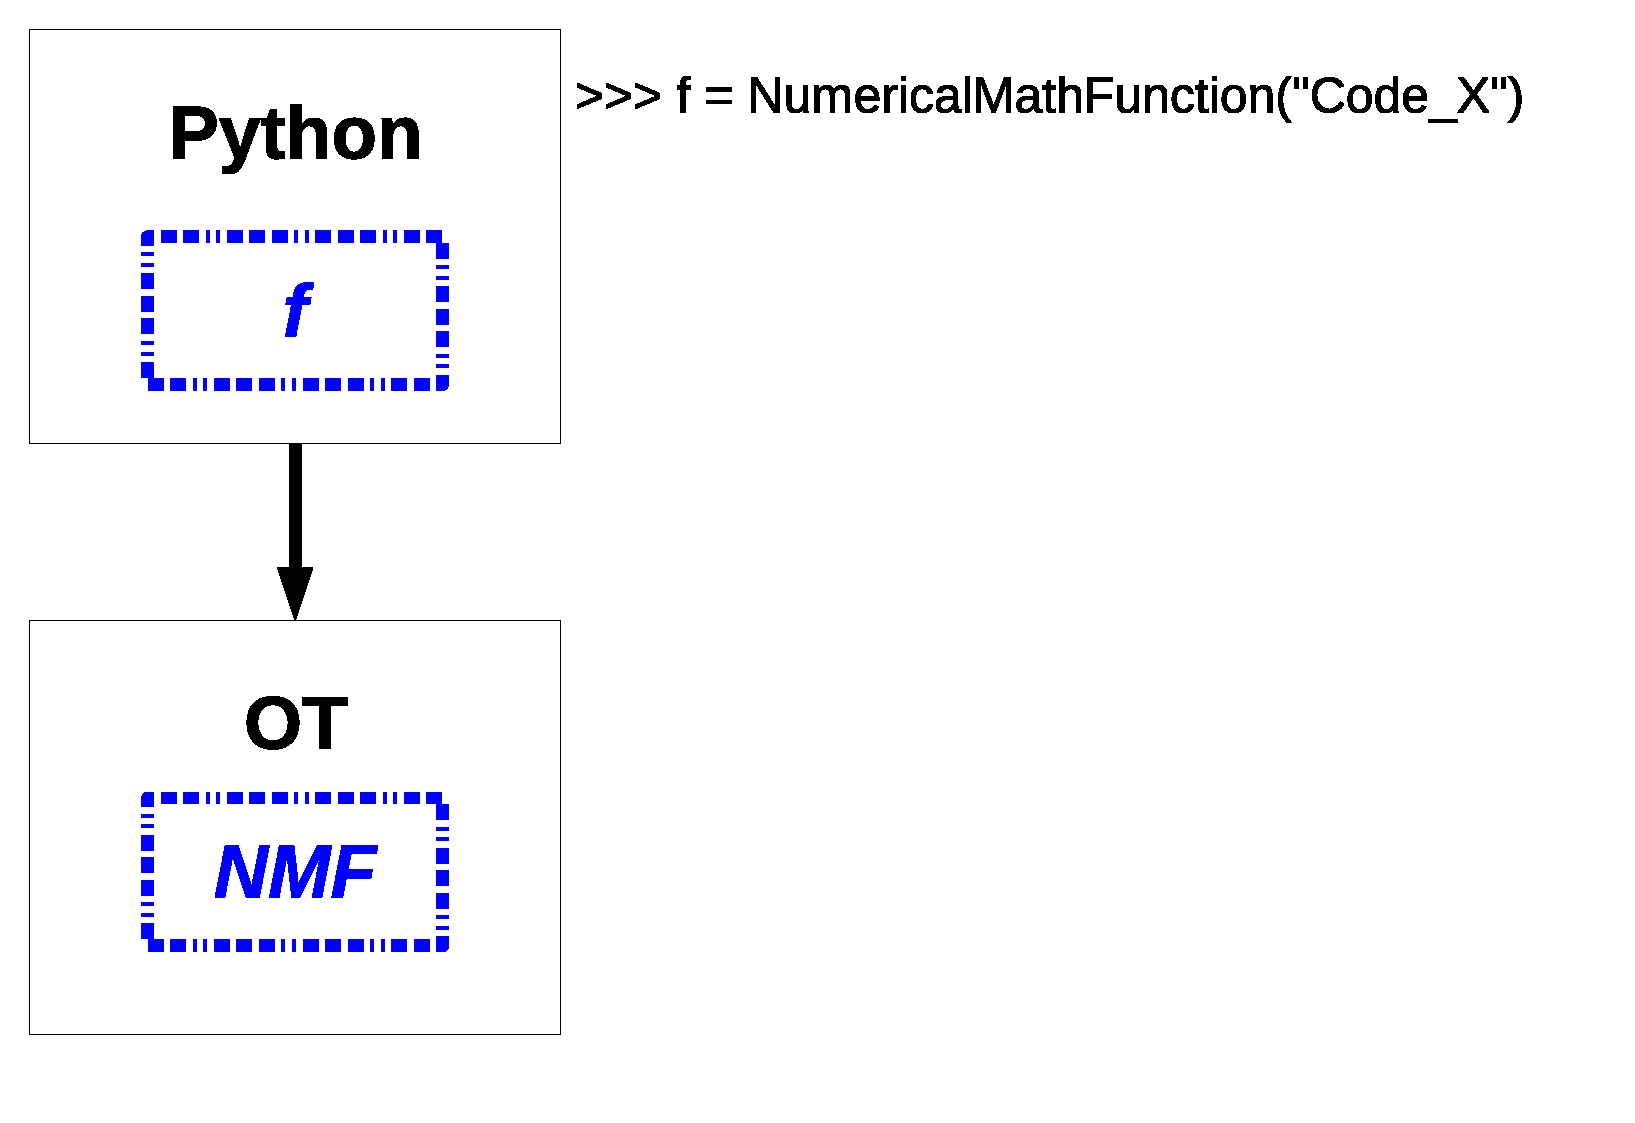
\includegraphics[width=12cm]{Figure3.pdf}
    \else
    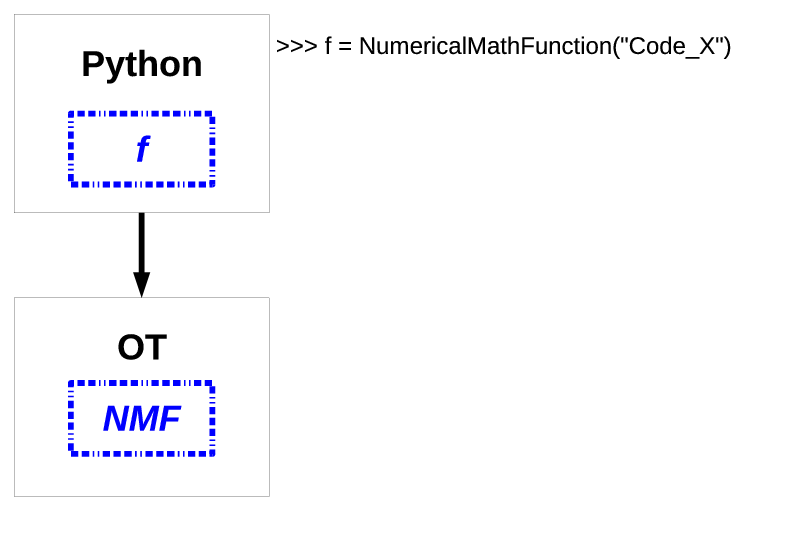
\includegraphics[width=12cm]{Figure3.png}
    \fi
    \caption[Figure 3]{Creating a \index{NumericalMathFunction}NumericalMathFunction}
  \end{center}
\end{figure}

\subsubsection{Step 2: Search for the \index{description file}description file}

The constructor of the \index{NumericalMathFunction}NumericalMathFunction class therefore receives a string which it interprets as the filename of the \index{wrapper}wrapper's XML \index{description file}description file (but without its {\bf .xml} extension). Thus the string {\bf Code\_X} matches the filename {\bf Code\_X.xml}.

After completing the name to restore its entirety, the file is searched on the computer's filesystem in a predefined list of directories (see Figure 3.4). These \index{wrapper search}directories are, in order:

\begin{enumerate}
\item those contained in the {\bf OPENTURNS\_WRAPPER\_PATH} environment variable, separated by a colon ({\bf :}) and read from left to right (if the variable does not exist or if its content is empty, this step is ignored);
\item the directory {\bf \$HOME/openturns/wrappers} if available;
\item the wrapper \index{installation}installation \index{installation directory}directory of the library, {\bf <openturns\_dir>/share/openturns/wrappers}, where {\bf <openturns\_dir>} is the installation directory of the \OT\ platform.
\end{enumerate}

If the file cannot be found, an error is generated and the {\bf f} object is not created, eg:

\index{NumericalMathFunction}\index{central term}
\lstset{language=Python, basicstyle=\normalsize}
\begin{lstlisting}[frame=TBRL]
  >>> f = NumericalMathFunction('NoFile')
  Traceback (most recent call last):
  File "<stdin>", line 1, in ?
  File "/local00/home/dutka/OpenTURNS/dutka/devel/build_3.4/install/lib/python2.
  4/site-packages/openturns/ot.py", line 11035, in __init__
  this = _ot.new_NumericalMathFunction(*args)
  RuntimeError: NoWrapperFileFoundException : FileNotFoundException : No file name
  d 'NoFile.xml' was found in any of those directories : /local00/home/dutka/opent
  urns/wrappers /local00/home/dutka/OpenTURNS/dutka/devel/build_3.4/install/share/
  openturns/wrappers
\end{lstlisting}

\begin{figure}
  \begin{center}
    \ifpdf
    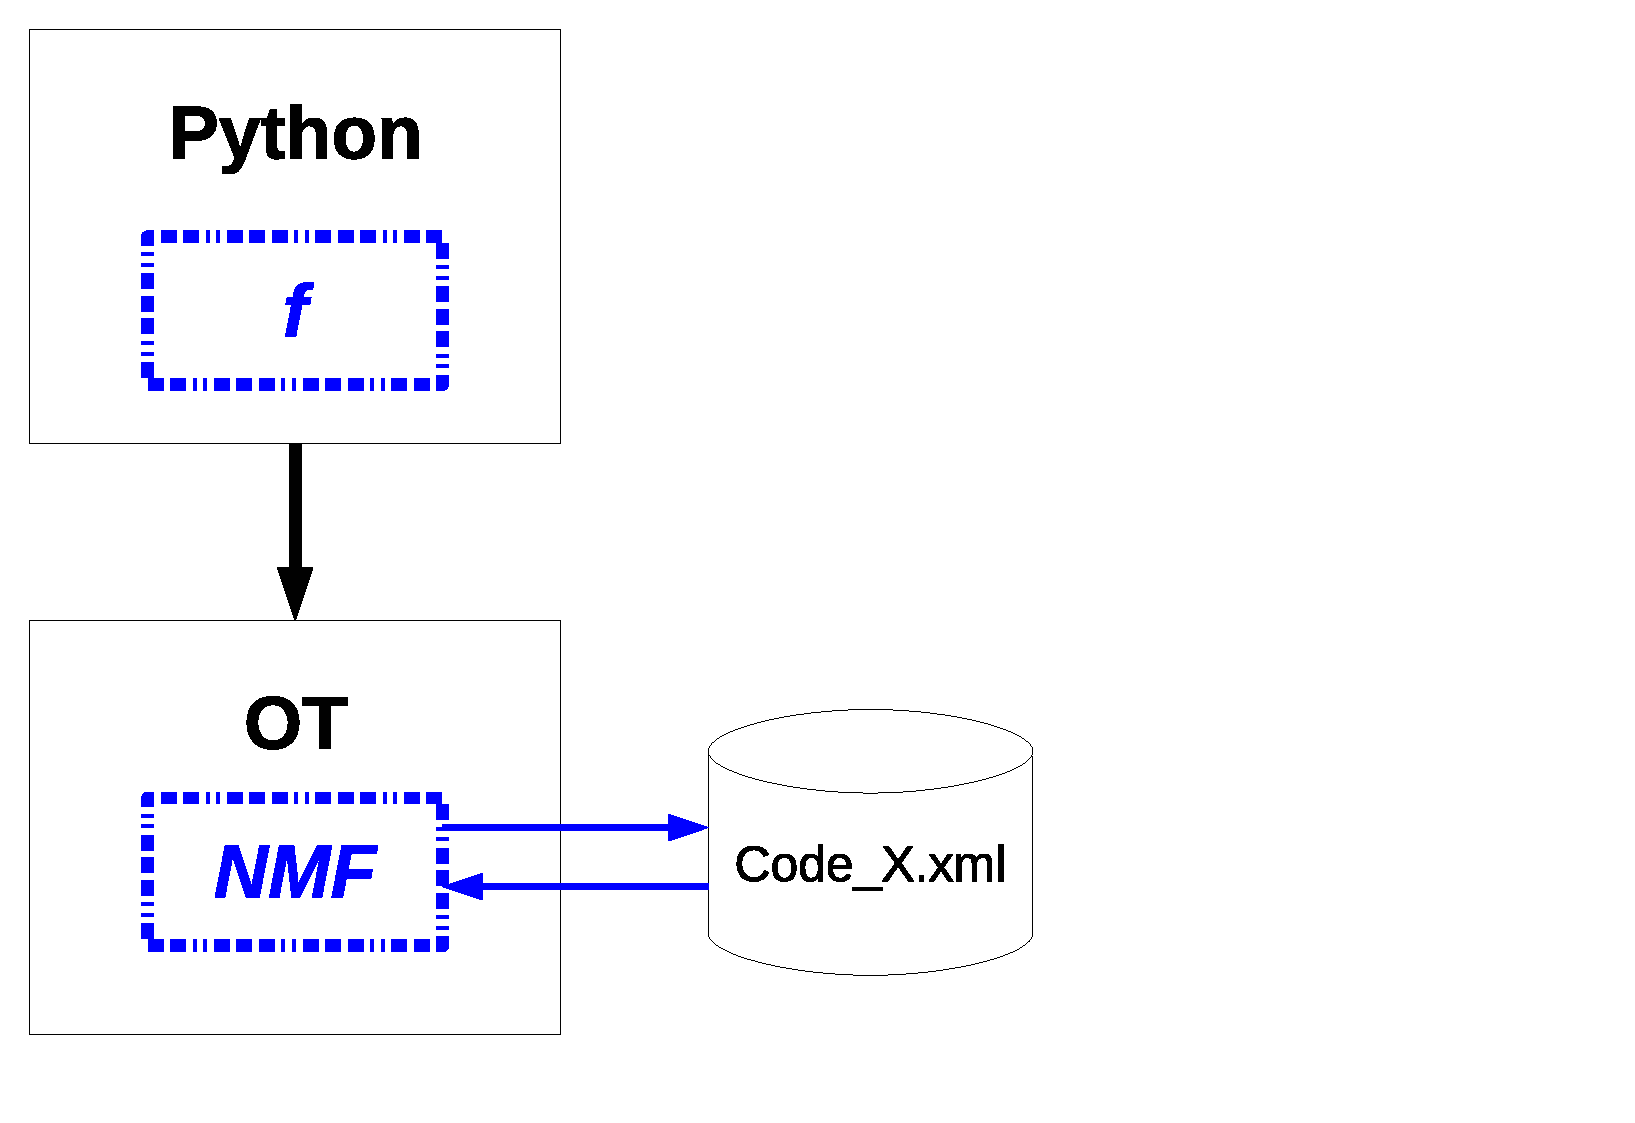
\includegraphics[width=12cm]{Figure4.pdf}
    \else
    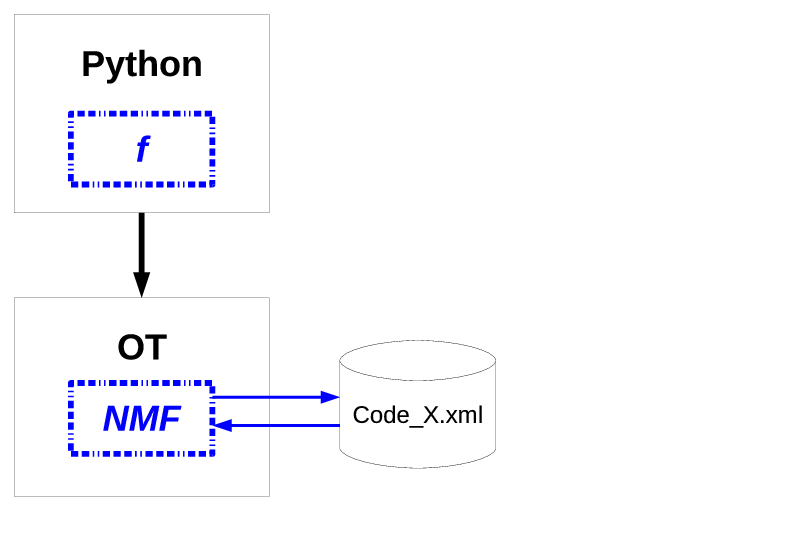
\includegraphics[width=12cm]{Figure4.png}
    \fi
    \caption[Figure 4]{Search of the \index{wrapper}wrapper's \index{description file}description file}
  \end{center}
\end{figure}

\subsubsection{Step 3: Analysis of the \index{description file}description file}

However, if the file is present, it is read. Any reading error causes a program error and the {\bf f} is not created. The details of this \index{description file}description file will be discussed later but, at this stage, it suffices to know that it contains the path to the {\bf Code\_X.so} \index{dynamic library}dynamic library (see Figure 3.5).

\begin{figure}
  \begin{center}
    \ifpdf
    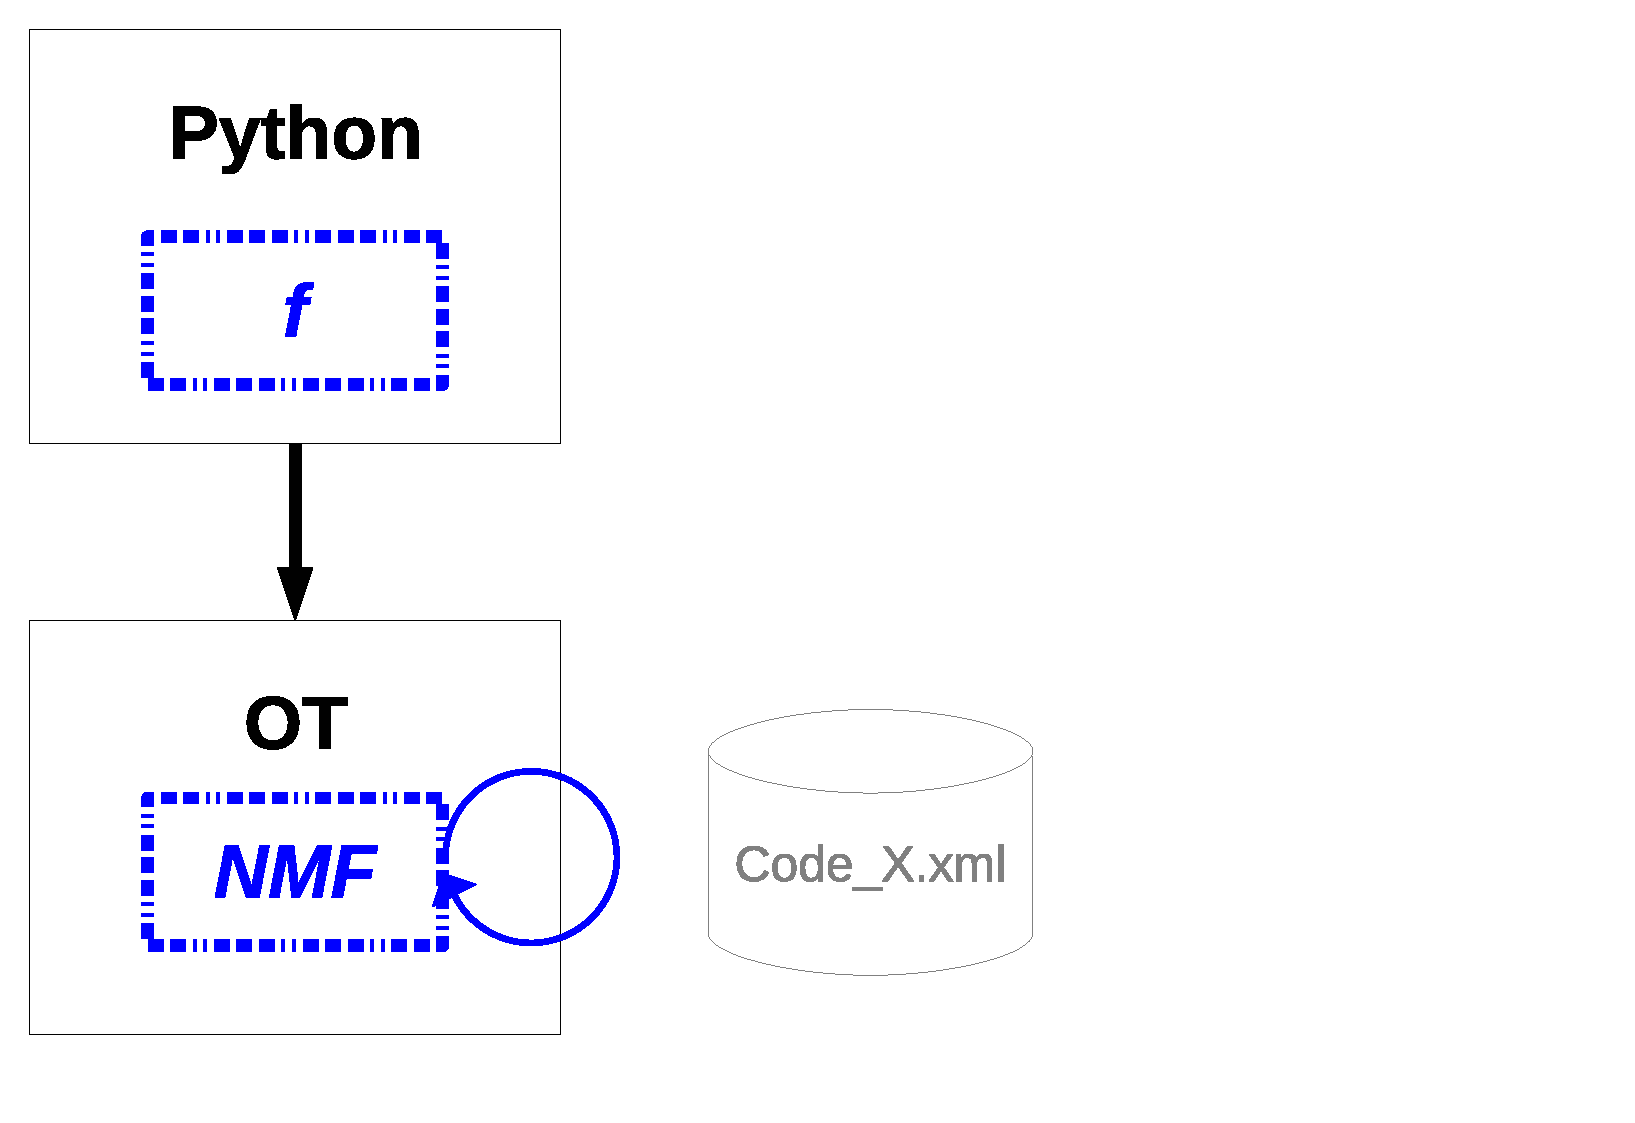
\includegraphics[width=12cm]{Figure5.pdf}
    \else
    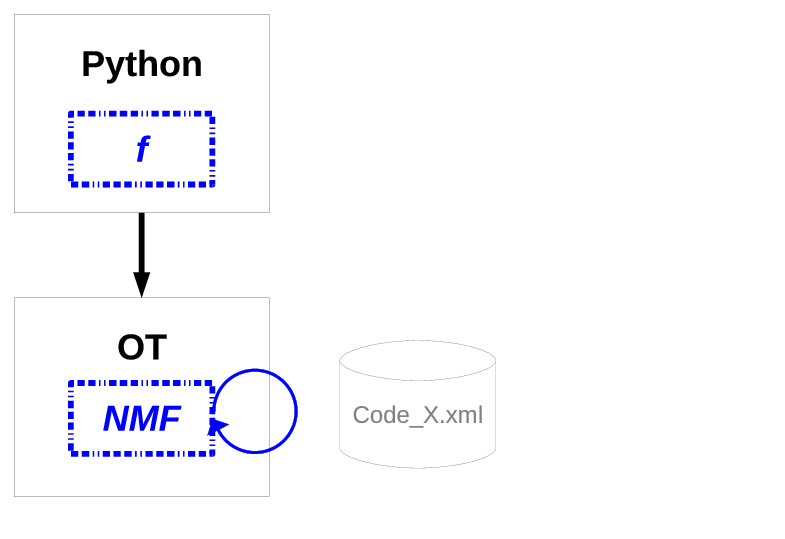
\includegraphics[width=12cm]{Figure5.png}
    \fi
    \caption[Figure 5]{Reading and analysis of the \index{wrapper}wrapper's \index{description file}description file}
  \end{center}
\end{figure}

\subsubsection{Step 4: Search for the \index{dynamic library}dynamic library}

In turn, this library will be searched for in the same directories. If it is found, it is automatically loaded by \OT (see Figure 3.6). Its absence causes an error.

\begin{figure}
  \begin{center}
    \ifpdf
    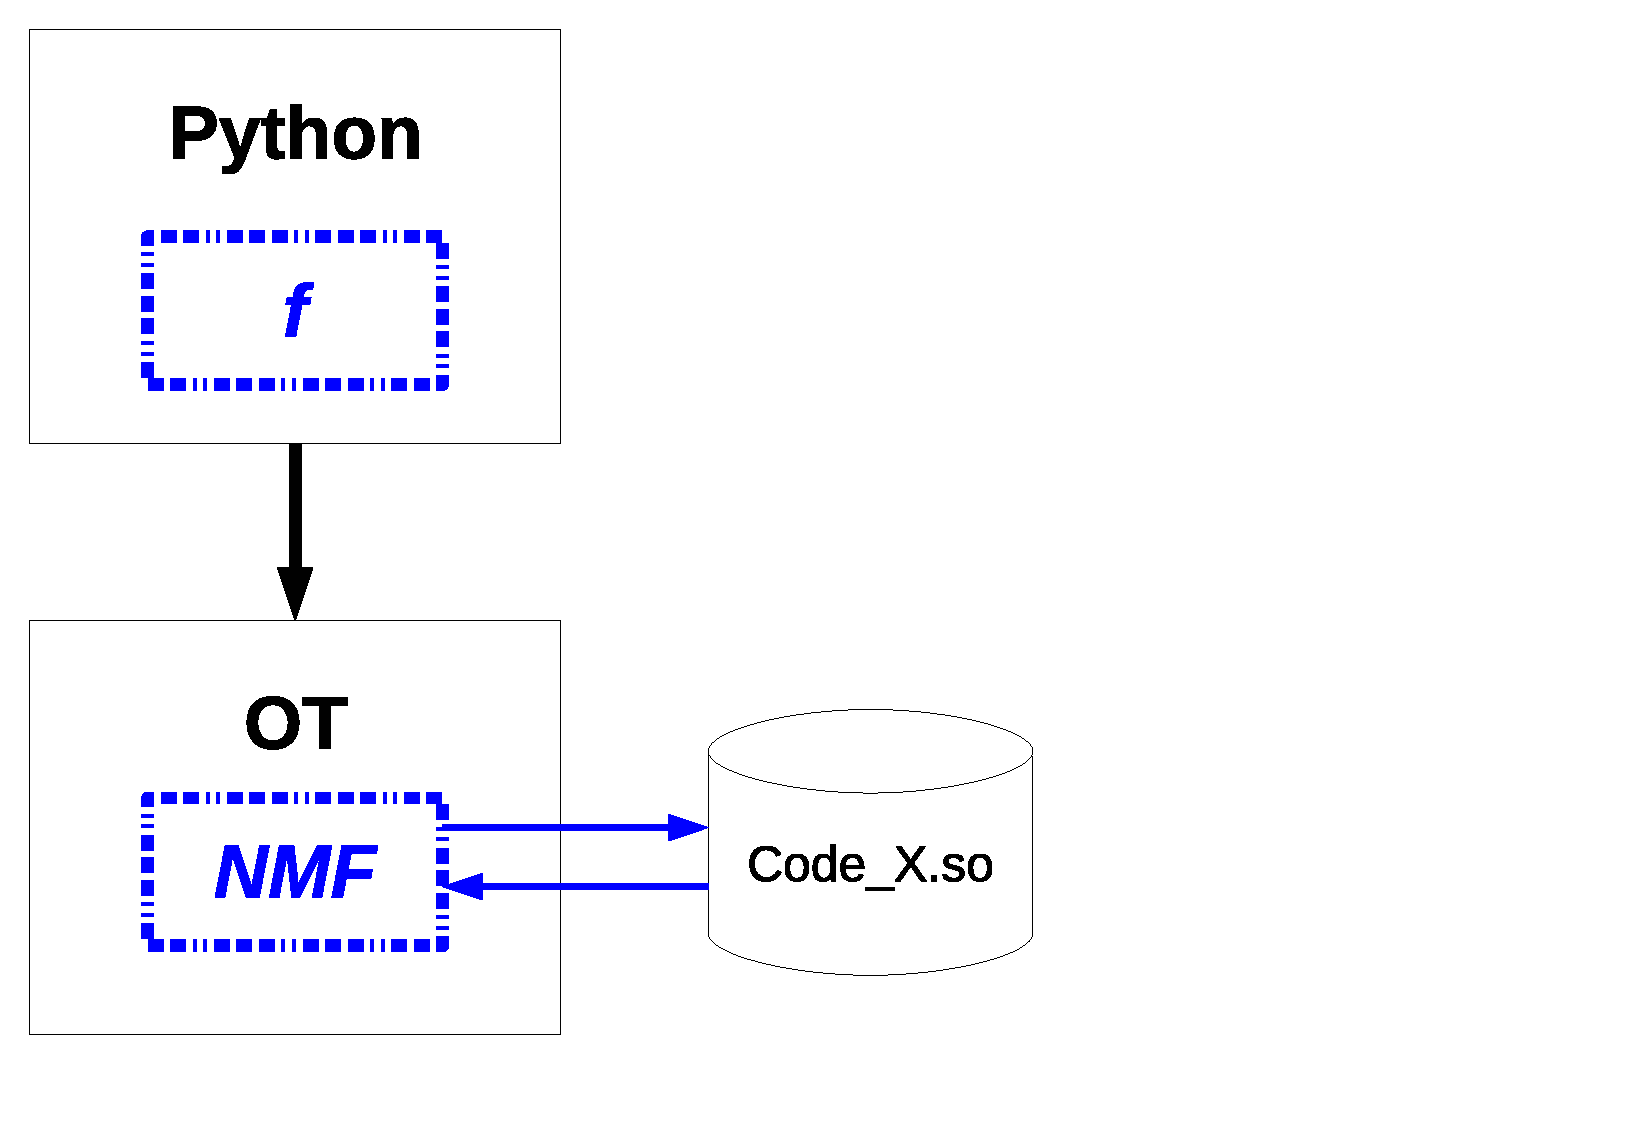
\includegraphics[width=12cm]{Figure6.pdf}
    \else
    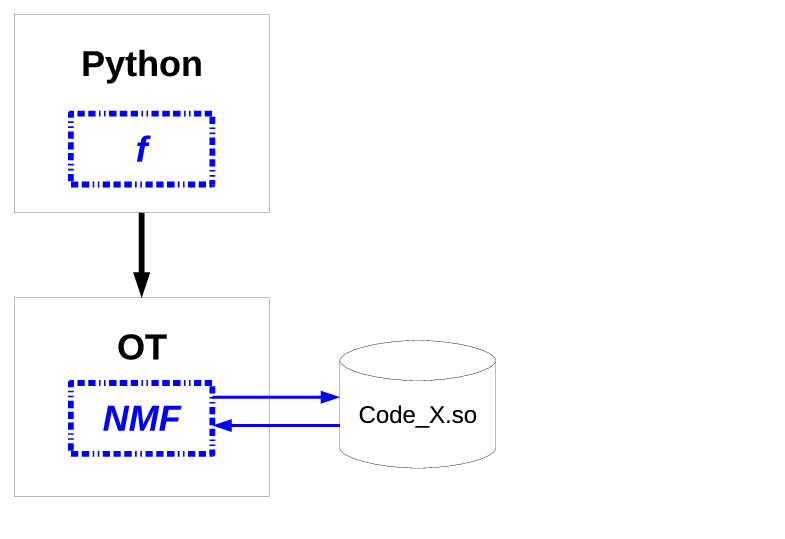
\includegraphics[width=12cm]{Figure6.png}
    \fi
    \caption[Figure 6]{Search for the \index{wrapper}wrapper's \index{dynamic library}dynamic library}
  \end{center}
\end{figure}

\subsubsection{Step 5: Loading the \index{dynamic library}dynamic library}

Once the library is loaded, it is tested to uncover some of its characteristics (see Figure 3.7). We will detail this \index{data structure}point in section 4.4.3, which deals with the {\bf getInfo\_}\footnote{At this stage of the document, the real names of the wrapper's functions have not been described yet. In fact, the \index{central term}{\bf getInfo\_} method carries a more elaborate name, with other elements as prefixes and suffixes. This will be described later on in the document. We will use the shortened name in order to simplify the text, as long as it does not raise any ambiguity.} method.

\begin{figure}
  \begin{center}
    \ifpdf
    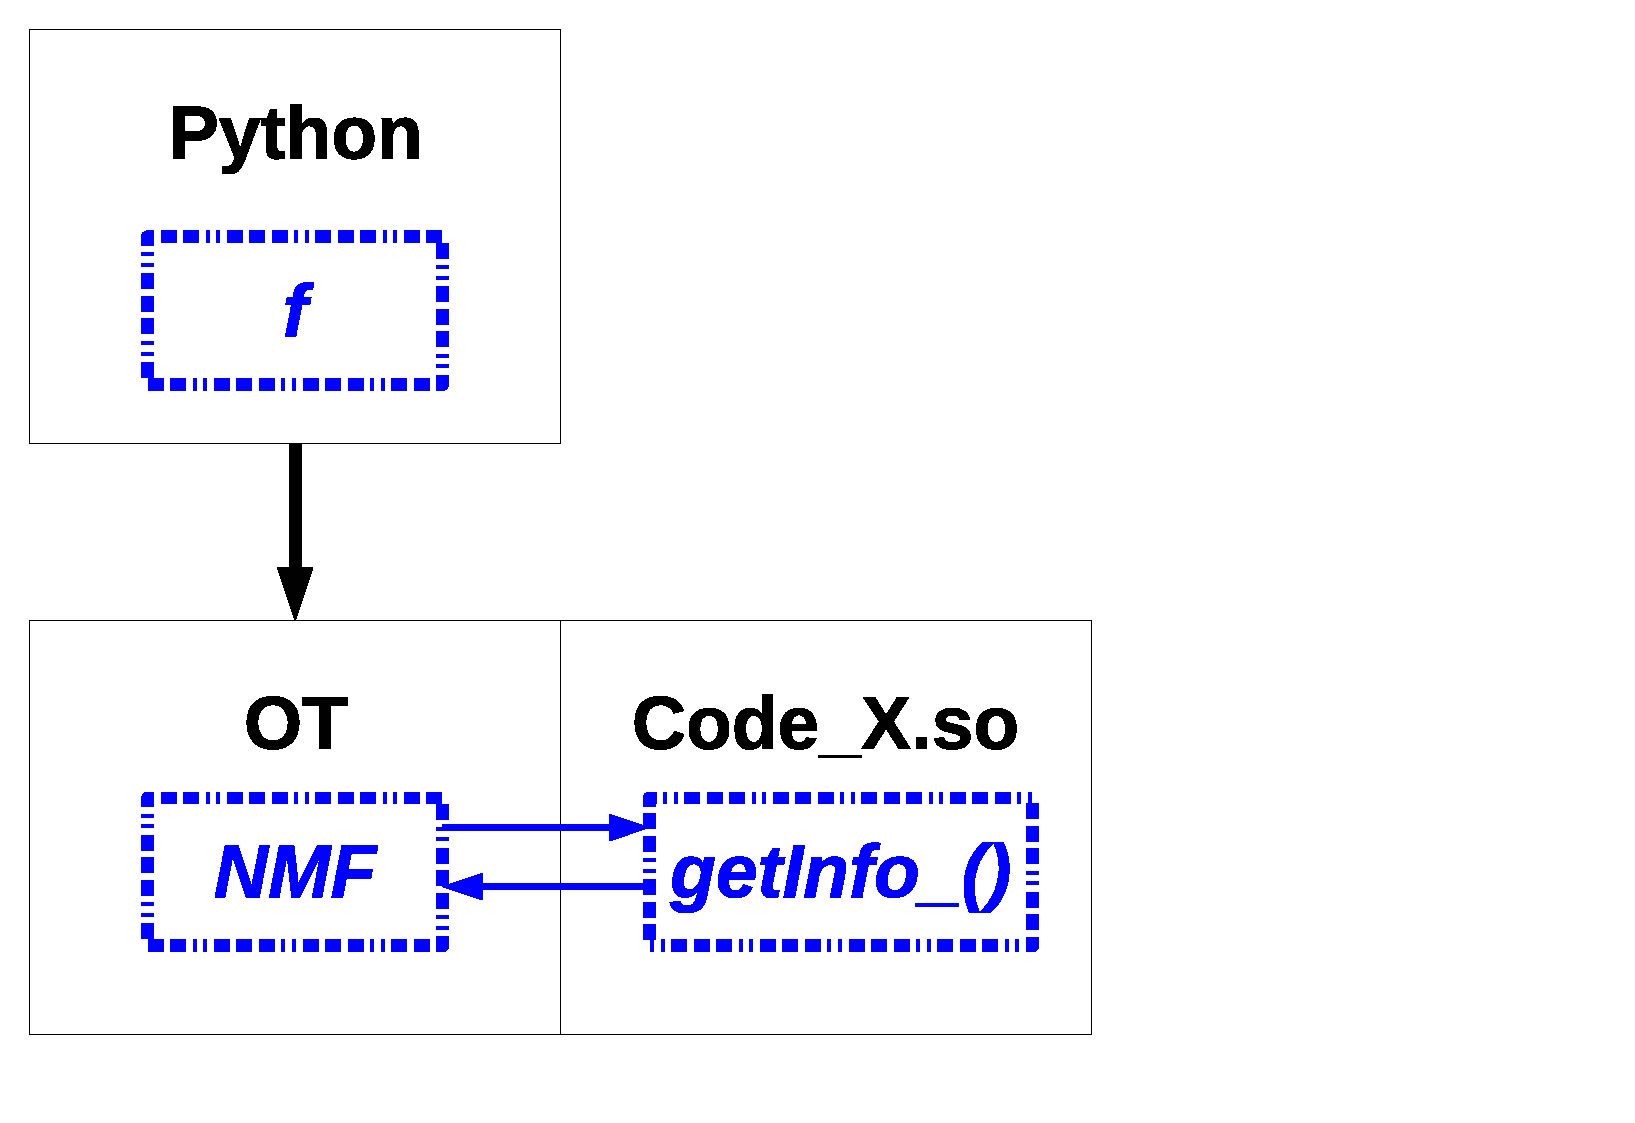
\includegraphics[width=12cm]{Figure7.pdf}
    \else
    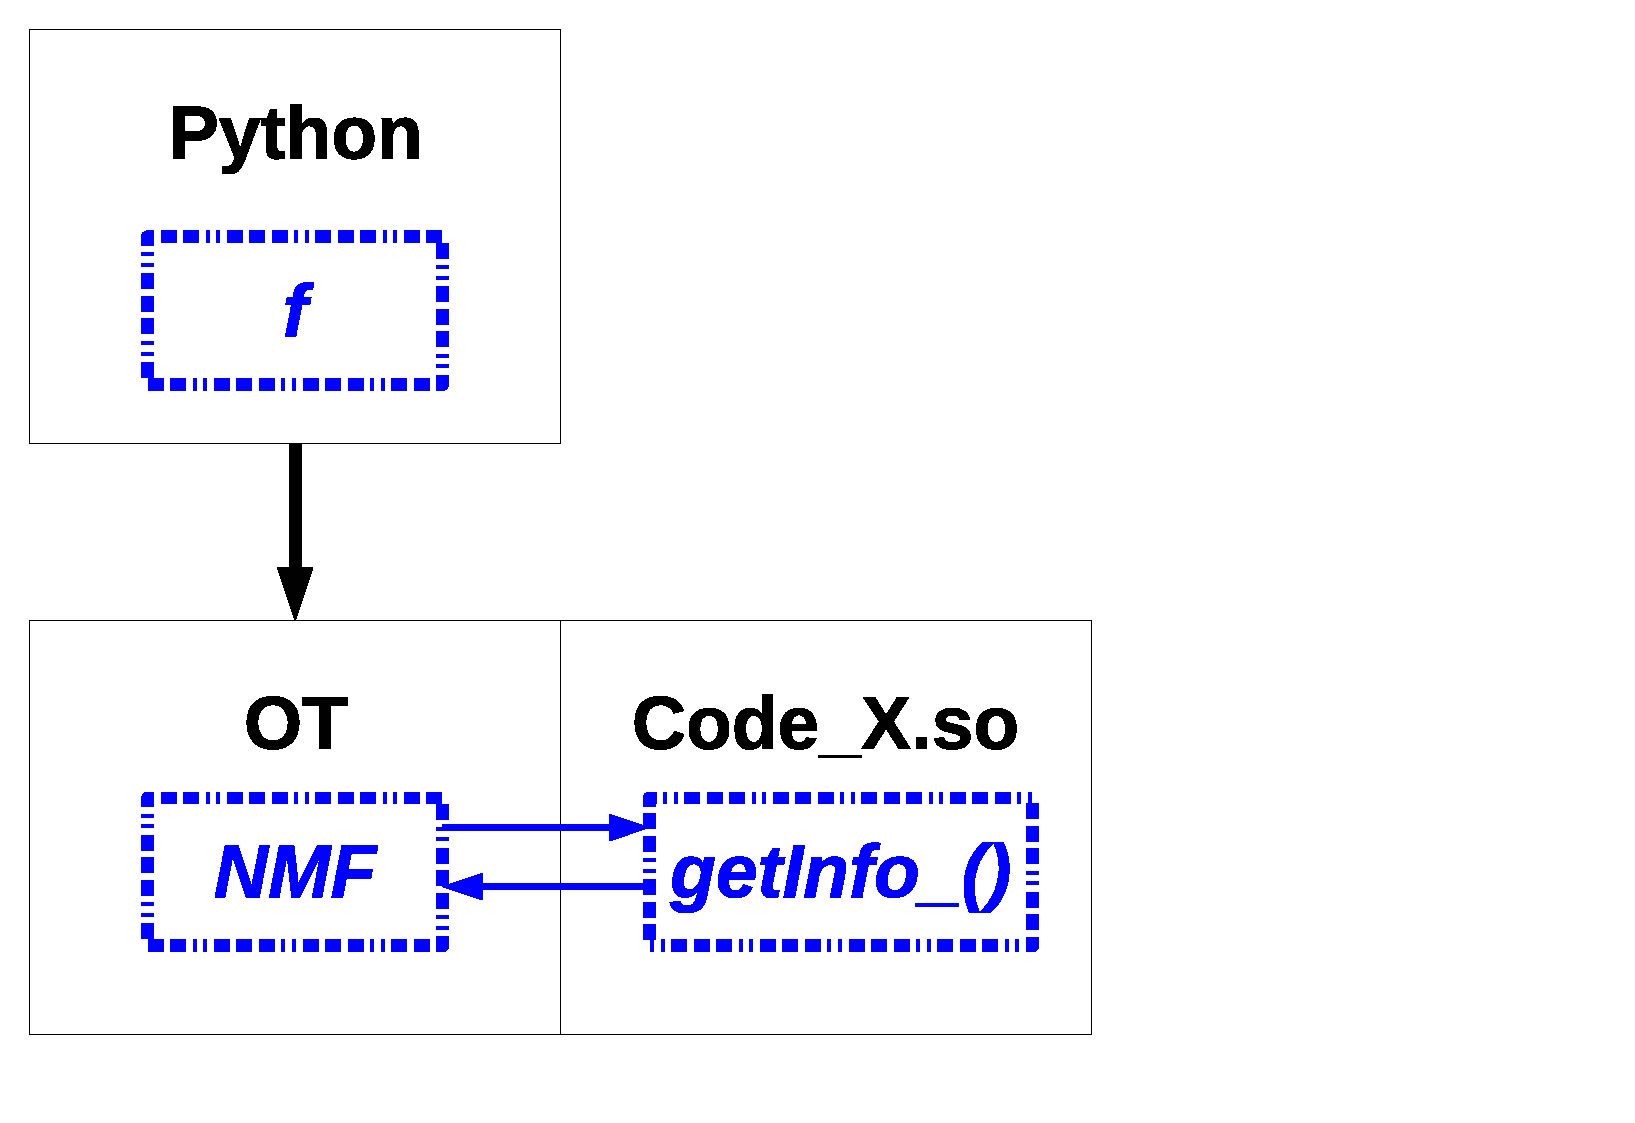
\includegraphics[width=12cm]{Figure7.pdf}
    \fi
    \caption[Figure 7]{Loading and querying the \index{dynamic library}dynamic library}
  \end{center}
\end{figure}

\subsubsection{Step 6: Completion of the \index{NumericalMathFunction}NumericalMathFunction construction}

Finally, \OT\ maintains an internal link to the \index{wrapper}wrapper's \index{dynamic library}dynamic library and returns a properly constructed and initialized \index{NumericalMathFunction}NumericalMathFunction object to the user (see Figure 3.8). It is therefore possible to use it for the study of uncertainties.

\begin{figure}
  \begin{center}
    \ifpdf
    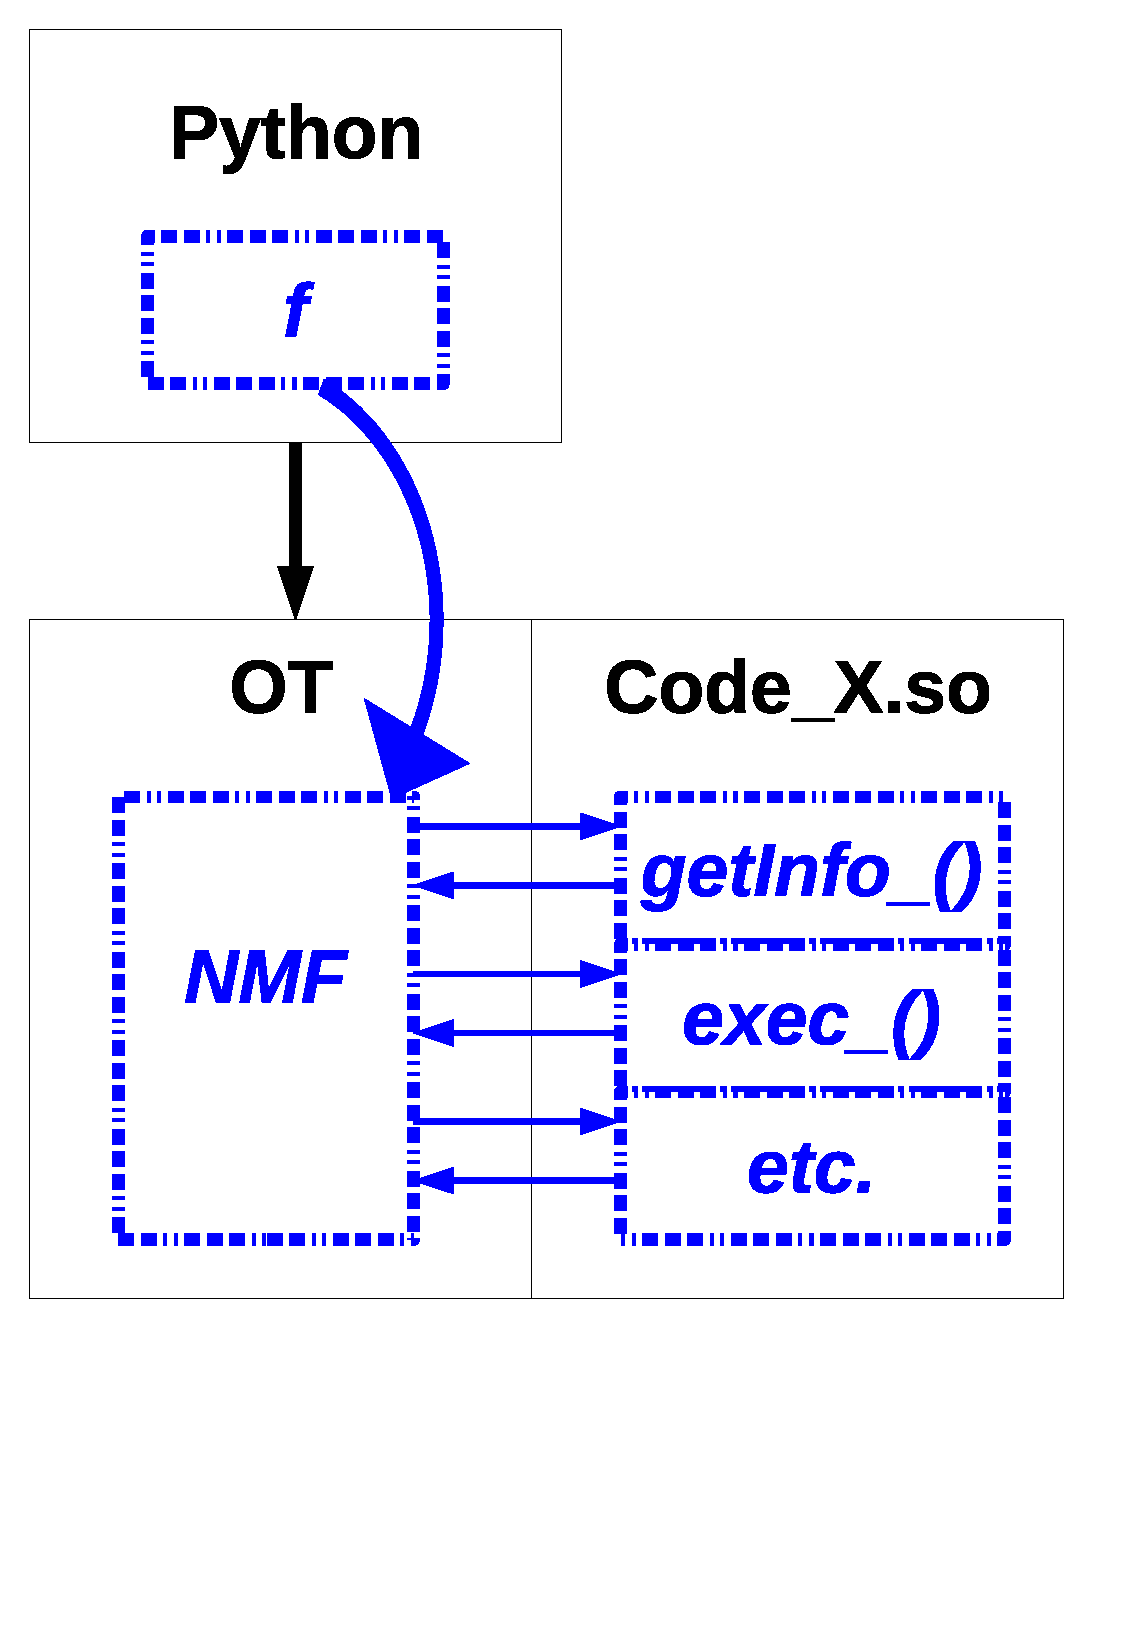
\includegraphics[height=12cm]{Figure8.pdf}
    \else
    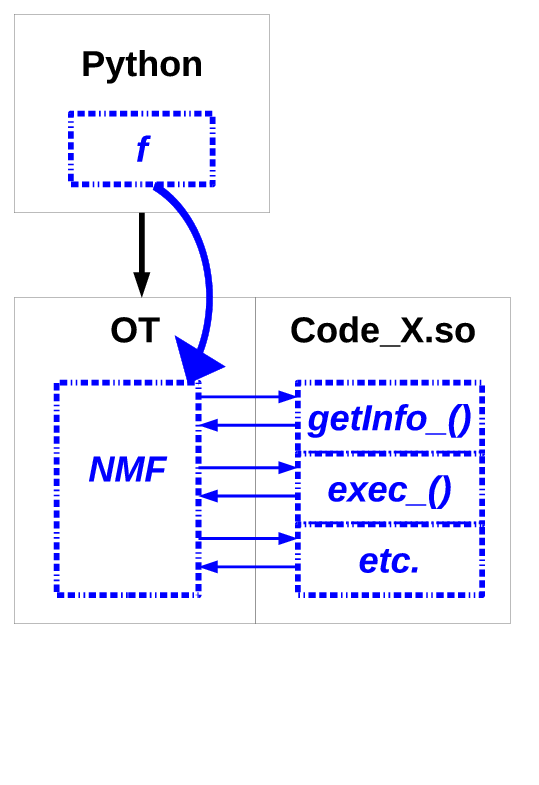
\includegraphics[height=12cm]{Figure8.png}
    \fi
    \caption[Figure 8]{Completion of the \index{NumericalMathFunction}NumericalMathFunction construction}
  \end{center}
\end{figure}

\subsection{Example: Creating a minimal \index{wrapper}wrapper}

To make this document more concrete, this section shows how to create a "minimal" \index{wrapper}wrapper. It will allow to browse the \index{description file}description file (see Section 3.2.4) and the source code in detail (see Section 3.2.5). It will especially help distinguish the elements that \emph{must} be present within any wrapper from elements that are optional and are only enriching features.

\subsubsection{Required Items}

In order not to unnecessarily complicate this first example, we will limit the \index{Function}Function implemented in the \index{wrapper}wrapper to a simple $\R^{3} \to \R^{2}$ analytical formula:

$$P\:\left\{\begin{array}{l}
    y_1 = x_1 \times e^{(- x_2 \times x_2)} \\
    y_2 = x_2 + x_3
  \end{array}\right.$$

We call this \index{Function}Function {\bf P}.

This \index{Function}Function is currently implemented directly in the \index{wrapper source code}source code of the \index{wrapper}wrapper. Later examples will show how this function can be extracted from the wrapper's body into an external code.

To create a \index{wrapper}wrapper based on {\bf P} which can be used by \OT, it is necessary to provide the library with the following elements:
\begin{itemize}
\item the path to the shared library that implements {\bf P}, {\bf P.so};
\item the list and description of variables exchanged between the \index{wrapper}wrapper and \OT, namely input variables ($x_1$, $x_2$ and $x_3$) and output variables ($y_1$ and $y_2$) of the \index{Function}Function;
\item the names of the \index{Function}Function within the \index{wrapper}wrapper, here {\bf P}, because the same wrapper can technically implement multiple Functions;
\item the name of the \index{Gradient}Gradient or the \index{Hessian}Hessian, if they are present in the \index{wrapper}wrapper, associated with the \index{Function}Function;
\item information on how P is implemented in the \index{wrapper}wrapper.
\end{itemize}

In our example, we will provide neither the \index{Gradient}Gradient nor the \index{Hessian}Hessian for {\bf P}, although this is quite feasible since P is very simple to derive. We will see later that the \OT\ library adapts itself and produces on its own a Gradient and a Hessian with centered finite differences.

\subsubsection{Starting from a template to generate the \index{wrapper}wrapper}

It is not easy, for a wrapper designer, to produce a first functional draft based on the analytical formula alone. Therefore, all versions of \OT\ offer by default a completely independent structure for wrapper development that allows to easily produce a wrapper.

Several development structures are offered in order to replace the old structure. The new structures are now available in the {\bf share/openturns/WrapperTemplates/<wrapper\_example>} subdirectory, where {\bf \index{wrapper}<wrapper\_example>} can be:
\begin{itemize}
\item {\bf wrapper\_calling\_shell\_command}: structure for the development of a wrapper launching the external code via a shell command line;
\item {\bf wrapper\_linked\_with\_C\_function}: structure for the development of a wrapper calling a C \index{function}function;
\item {\bf wrapper\_linked\_with\_F77\_function}: structure for the development of a wrapper calling a \index{FORTRAN}FORTRAN 77 \index{function}function.
\end{itemize}

We copy the {\bf \index{wrapper}wrapper\_linked\_with\_C\_function directory} as {\bf Pwrapper}:

\index{installation directory}
\lstset{language=Bash, basicstyle=\normalsize}
\begin{lstlisting}[frame=TBRL]
  > cp -r <openturns_dir>/share/openturns/WrapperTemplates/wrapper_linked_with_C
  _function $HOME/Pwrapper
\end{lstlisting}

Then, just use the {\bf customize} script which automatically renames the files with the name passed as an argument:

\lstset{language=Bash, basicstyle=\normalsize}
\begin{lstlisting}[frame=TBRL]
  > ./customize P
\end{lstlisting}

\subsubsection{Compilation and \index{installation}installation of the \index{wrapper}wrapper}

Before going into detail on how to write the wrapper, we need to prepare the development environment which will conduct the \index{compilation}compilation and installation of the library and of its XML file.

\small
\begin{quote}
  \textit{Note: To be able to use the {\bf Pwrapper} user development directory, the developer must have access to three GNU Open Source tools known as {\bf autoconf}, {\bf automake} and {\bf libtool}. These tools are commonly installed on all GNU/Linux distributions. However the installed versions may be older and it is always good to have the latest available update\footnote{See the website {\bf http://www.openturns.org} to check the tool versions adapted to the \OT\ version you are using.}.\\
    The user must also have a C or C++ compiler in order to produce the \index{wrapper}wrapper's \index{dynamic library}dynamic library. The GNU Open Source compiler {\bf gcc} is a very good choice.}
\end{quote}
\normalsize

The first step is to bootstrap the environment. To this end, the following command must be executed once:

\lstset{language=Bash, basicstyle=\normalsize}
\begin{lstlisting}[frame=TBRL]
  > bootstrap
\end{lstlisting}

Then we determine which tools are available on the computer in order to compile and install the \index{wrapper}wrapper. This configuration step is also carried out only once:

\index{installation directory}
\lstset{language=Bash, basicstyle=\normalsize}
\begin{lstlisting}[frame=TBRL]
  > ./configure --with-openturns=<openturns_dir>
\end{lstlisting}

By default, the \index{wrapper}wrapper is installed in the directory {\bf \$HOME/openturns/wrappers} which is a standard search directory of \OT.

\small
\begin{quote}
  \textit{Note: If the wrapper must be installed in a different directory, it is necessary to use the option {\bf --prefix = <Pwrapper\_dir>} where {\bf <Pwrapper\_dir>} is the directory where the wrapper will be installed (later on). When using the wrapper, the path to {\bf <Pwrapper\_dir>} should be positioned in the environment variable \index{wrapper search}{\bf OPENTURNS\_WRAPPER\_PATH}.}
\end{quote}
\normalsize

When the source files needed to produce the \index{wrapper}wrapper are written (see sections 3.2.4 and 3.2.5), it will be possible to compile and then install the wrapper using the commands:

\lstset{language=Bash, basicstyle=\normalsize}
\begin{lstlisting}[frame=TBRL]
  > make
  > make install
\end{lstlisting}

\subsubsection{\index{description file}Description file for the minimal \index{wrapper}wrapper}

We begin by writing, or rather by modifying the description file {\bf P.xml}.

This XML file is highly structured and must contain a certain number of tags. This rigid syntax is checked by a grammar (\index{DTD}DTD) described in the \index{wrapper}{\bf wrapper.dtd} file. This DTD is provided by default by \OT\footnote{The file should normally be found in the {\bf <openturns\_dir>/share/openturns/wrappers} directory.}. Any error in the syntax or the structure of the XML file results in immediate rejection by the \OT\ library and prevents from loading the wrapper.

The {\bf P.xml} file contains the following tags:

\begin{description}
\item[<wrapper>] \index{wrapper}This tag introduces the general description of the wrapper.

\item[<library>] This tag introduces the section dealing with the \index{dynamic library}dynamic library as seen from the \OT standpoint.

\item[<path>] This tag allows to indicate to \OT\ where to find the wrapper's dynamic library, {\bf P.so} in our convention. It thus reads:

  \lstset{language=XML, basicstyle=\normalsize}
  \begin{lstlisting}[frame=TBRL]
    <wrapper>
    <library>
    <path>P.so</path>
    ...
  \end{lstlisting}

  The name of the \index{dynamic library}dynamic library is marked by the opening tag {\bf <path>} and the closing tag {\bf </path>} following the standard XML syntax. Be careful not to introduce whitespaces or any other separator, for all characters between the opening and closing tags \emph{will} be considered as the library name. The library will be sought in the same directory as the XML file (see Section 3.1.3) because the system assumes that both files are placed in the same directory.

  If the library name is preceded by a relative path, this path will be relative to the above-mentioned search directories. Absolute paths are relative to the computer's file system.

\item[<description>] This tag introduces the definition of the \index{Function}Function, the \index{Gradient}Gradient, the \index{Hessian}Hessian and of the exchanged variables.

\item[<variable-list>] This tag introduces the list of input and output variables of the \index{wrapper}wrapper.

\item[<variable>] This tag allows to define a wrapper input or output variable  as shown in the following example.

  \lstset{language=XML, basicstyle=\normalsize}
  \begin{lstlisting}[frame=TBRL]
    ...
    <description>
    <variable-list>

    <!-- three input variables -->
    <variable id="x1" type="in" />
    <variable id="x2" type="in" />
    <variable id="x3" type="in" />

    <!-- two output variables -->
    <variable id="y1" type="out" />
    <variable id="y2" type="out" />

    </variable-list>
    ...
  \end{lstlisting}

  It is used to declare the three input variables ({\bf x1}, {\bf x2} and {\bf x3}) and two output variables ({\bf y1} and {\bf y2}) of the {\bf P} \index{Function}Function. The {\bf id} attribute specifies the variable name and the {\bf type} attribute, its nature ({\bf in} for input and {\bf out} for output, from the point of view of {\bf P}). We remind here that the exchanged variables are doubles.

  It is a good practice to list the variables in their natural order, input before output. This order is used internally by \OT\ so as to determine to which variable it must assign the values of the input and output point components when evaluating the Function. Thus, the first component of the point\index{data structure} will be assigned to the first listed variable, the second component to the second listed variable, and so on.

  Each variable must have a unique identifier ({\bf id}). If this is not the case, the \index{description file}description file is rejected.

  We will see later on that the {\bf <variable>} tags may be supplemented by sub-tags providing additional information.

\item[<function>, <gradient>, <hessian>] These three tags are used to respectively define the names of the \index{Function}Function, the \index{Gradient}Gradient and the \index{Hessian}Hessian. In our example of a minimal \index{wrapper}wrapper, only the Function is defined under the name {\bf P}. The name is written between the opening and closing tags without spaces or any other superfluous character.

  \lstset{language=XML, basicstyle=\normalsize}
  \begin{lstlisting}[frame=TBRL]
    ...
    <function provided="yes">P</function>
    <gradient provided="no" />
    <hessian  provided="no" />
    </description>
    </library>
    ...
  \end{lstlisting}

  The {\bf <function>}, {\bf <gradient>} or {\bf <hessian>} tags include a {\bf provided} attribute that indicates whether the Function, the Gradient or the Hessian is implemented in the wrapper ({\bf yes}) or not ({\bf no}). In the latter case, the name need not be specified.

\item[<external-code>] This tag introduces the definition of the coupling between the wrapper and the external code.

\item[<data>] This tag introduces the definition of the data exchanged between the wrapper and the external code. In our minimal example, there really is no external code since the wrapper will play this role without resorting to some other object. This section will therefore remain empty.
\end{description}

The remaining information to be given to \OT\ deals with the way the \index{wrapper}wrapper internally implements the \index{Function}Function. The presence of this information is justified for the development of a generic wrapper, but is useless in the example at hand. Yet it is still necessary to provide these pieces of information in order to have a valid \index{description file}description file. Future developments of \OT\ will eliminate this dependence.

\begin{description}
\item[<wrap-mode>] This tag indicates the way the \index{wrapper}wrapper internally implements the \index{Function}Function.

  The {\bf type} attribute indicates that the Function is directly coded within the wrapper ({\bf static-link}). The sub-tags {\bf <in-data-transfer>} and {\bf<out-data-transfer>} specify that the variables must be passed to the Function as arguments.

\item[<command>] This tag describes the system command that calls the external code when it is fully independent and disjoint from the wrapper. Here, since the wrapper is minimal, no command is defined.

  \lstset{language=XML, basicstyle=\normalsize}
  \begin{lstlisting}[frame=TBRL]
    ...
    <external-code>
    <data />

    <wrap-mode type="static-link">
    <in-data-transfer  mode="arguments" />
    <out-data-transfer mode="arguments" />
    </wrap-mode>

    <command />

    </external-code>
    </wrapper>
  \end{lstlisting}
\end{description}

Finally, the \index{description file}description file {\bf P.xml.in} for our minimal \index{wrapper}wrapper looks like this:\index{DTD}
\lstset{language=XML, basicstyle=\normalsize}
\begin{lstlisting}[frame=TBRL]
  <?xml version="1.0" encoding="ISO-8859-1"?>
  <!DOCTYPE wrapper SYSTEM "@OPENTURNS_WRAPPER_DTD_PATH@/wrapper.dtd">

  <wrapper>
  <library>
  <path>P.so</path>
  <description>
  <variable-list>
  <variable id="x1" type="in"  />
  <variable id="x2" type="in"  />
  <variable id="x3" type="in"  />
  <variable id="y1" type="out" />
  <variable id="y2" type="out" />
  </variable-list>
  <function provided="yes">P</function>
  <gradient provided="no" />
  <hessian  provided="no" />
  </description>
  </library>
  <external-code>
  <data />
  <wrap-mode type="static-link">
  <in-data-transfer  mode="arguments" />
  <out-data-transfer mode="arguments" />
  </wrap-mode>
  <command />
  </external-code>
  </wrapper>
\end{lstlisting}

\subsubsection{Source code for the minimal \index{wrapper source code}wrapper}

The second file needed to produce the \index{wrapper}wrapper is the source code of the \index{dynamic library}dynamic library ({\bf wrapper.c}).

This source code is used to carry out the interface adaptation required by the data transfer between \OT\ and the \index{Function}Function to implement. It could theoretically be written in any language evolved enough to perform such operations. But the fact that the \index{wrapper}wrapper's library is dynamically loaded, and that \OT\ must search for symbols in it and be able to call them, requires the use of a computer interface based on C. This sets strong constraints on the languages that can be used to code the wrapper. Only C and C++ are easily usable for this task.

\small
\begin{quote}
  \textit{Note: This constraint does not mean that the developer should be a C or C++ expert to be able to develop a wrapper. The engineering work done in \OT\ helped greatly simplify the writing of the wrapper, and any developer used to a procedural language (\index{FORTRAN}FORTRAN or other) is able to generate a wrapper. However, they must obey the rules imposed by \OT.}
\end{quote}
\normalsize

The first thing to do, in the \index{wrapper source code}source file {\bf wrapper.c}, is to include the header file which provides definitions needed for \index{compilation}compilation:\index{Wrapper.h}

\lstset{language=C, basicstyle=\normalsize}
\begin{lstlisting}[frame=TBRL]
  #include "Wrapper.h"
  ...
\end{lstlisting}

These two files are provided by default in the \OT\ \index{installation}installation.

The file {\bf Wrapper.h} is absolutely essential and should always be included in the source code of the wrapper. It gathers all the definitions that allow communication between the \OT\ library and the wrapper. Without this file, no compilation of the wrapper is possible.

It also contains the declarations of functions that are practical and shared by many wrappers. These functions are part of the platform with which the wrapper connects itself. The use of these functions greatly simplifies the writing of wrappers by performing the most common actions in a simple and efficient way. This documentation largely relies on them. The first appendix describes the functions in this library.

Let's recall the definition of our {\bf P} \index{Function}Function:

$$P\:\left\{\begin{array}{l}
    y_1 = x_1 \times e^{(- x_2 \times x_2)} \\
    y_2 = x_2 + x_3
  \end{array}\right.$$

Among the different techniques available to implement the {\bf P} Function in the \index{wrapper}wrapper, we choose to isolate the computation in a separate C \index{function}function which we call {\bf myP}. The function being multidimensional $\R^{3} \to \R^{2}$, the C function has been designed to accept an array of 3 doubles as input and an array of 2 doubles as output.

We assume that the arrays are already allocated with the proper size (respectively $n$ and $p$) and that only the output values are to be modified.

We also use the C function return value to indicate a possible miscalculation. Here, since the calculation is always possible, the function systematically returns 0 to indicate that no error occurred (this is a C convention). In case of an error, such as a division by zero or an argument outside the Function's definition domain, the function needs to return a non-zero return code.

\lstset{language=C, basicstyle=\normalsize}
\begin{lstlisting}[frame=TBRL]
  ...
  #include <math.h>

  int myP ( double * x, unsigned long n,
  double * y, unsigned long p )
  {
    y[0] = x[0] * exp( - x[1] * x[1] );
    y[1] = x[1] + x[2];
    return 0;
  }
  ...
\end{lstlisting}

In the example, we used the names {\bf x} and {\bf y} to refer to the input variables ({\bf x1}, {\bf x2} and {\bf x3}) and output variables ({\bf y1} and {\bf y2}). However, seing that the C language requires to start numbering array indices from zero: {\bf x[0]} corresponds to {\bf x1}, {\bf x[1]} to {\bf x2}, etc.

\small
\begin{quote}
  \textit{Note: Inclusion of the {\bf math.h} file is justified by the use of the {\bf exp} \index{function}function.}
\end{quote}
\normalsize

Having this {\bf P} \index{Function}Function, we now need to interface it with \OT. This is done using an auxiliary \index{function}function that will ensure communication with the \OT\ library.

This function is commonly called \index{central term}{\bf exec\_}, although its name is more complex as shown by the following example:

\index{prefix}\index{internal state}\index{data structure}
\lstset{language=C, basicstyle=\normalsize}
\begin{lstlisting}[frame=TBRL]
  ...
  enum WrapperErrorCode func_exec_P ( void * p_state,
  const struct point * inPoint,
  struct point * outPoint )
  {
    if ( myP (inPoint->data_,  inPoint->size_,
    outPoint->data_, outPoint->size_ ) ) return WRAPPER_EXECUTION_ERROR;

    return WRAPPER_OK;
  }
\end{lstlisting}

The \index{central term}{\bf exec\_} \index{function}function is responsible for calling the previously written {\bf myP} function and passing to it the ad-hoc arguments that it will search within the data structures passed as arguments. These data structures are already allocated and filled (for those who may be) so that the functions of the \index{wrapper}wrapper simply have to fill them. No memory management is to be performed at this level in the wrapper, which makes it very simple to use.

We have seen that the {\bf myP} \index{function}function could, in case of failure, warn the calling code about it. This case is treated by the test ({\bf if}) which returns a {\bf WRAPPER\_EXECUTION\_ERROR} error code to \OT. Otherwise the \index{return code}{\bf WRAPPER\_OK} code indicates that everything went smoothly.

\subsubsection{Checking if the minimal \index{wrapper}wrapper is functioning}

This being written, we saw that we only needed to compile and install the wrapper to run it (see sections 3.2.2 and 3.2.3). If the wrapper was installed in a standard \OT\ directory or if the \index{wrapper search}{\bf OPENTURNS\_WRAPPER\_PATH} environment variable was correctly set, it is possible to test its basic operation by using a small Python script (eg {\bf test\_P.py}) which is executed as follows:

\lstset{language=Bash, basicstyle=\normalsize}
\begin{lstlisting}[frame=TBRL]
  > python test_P.py
\end{lstlisting}

Congratulations! You have written the smallest possible wrapper and you have interfaced it with \OT.

After loading the entire \OT\ library ({\bf import}), the script creates a \index{NumericalMathFunction}NumericalMathFunction type object ({\bf P}) which loads the \index{wrapper}wrapper that we just built. It then evaluates this P object by passing a NumericalPoint ({\bf x}) to it as an argument. This action causes the \index{execution}execution of the C \index{function}function {\bf myP}, computing the analytical formula written in the source code of the \index{wrapper source code}wrapper, and the return of the value of the computed \index{NumericalMathFunction}NumericalPoint ({\bf y}).

Essentially, the script {\bf test\_P.py} carries out the following series of actions:

\lstset{language=Python, basicstyle=\normalsize}
\begin{lstlisting}[frame=TBRL]
  >>> from openturns import *
  >>> P = NumericalMathFunction ( "P" )
  >>> x = NumericalPoint ( 3 )
  >>> x[0] = 10.
  >>> x[1] = 20.
  >>> x[2] = 30.
  >>> print x
  [...]
  >>> y = P ( x )
  >>> print y
  [...]
\end{lstlisting}
